\documentclass{article}

% Add custom.sty from the main directory
\usepackage{../../custom}

\title{Homework 3 - Segmentation and Homography}
\author{Naomi Derel, 325324994 
\and Sagi Ben Lulu, 207031493}
\date{08.01.2025}

\begin{document}

\maketitle

\section*{Question 3 - Planar Homographies}

\subsection*{3.0 - SIFT}

\begin{figure}[h!]
    \centering
    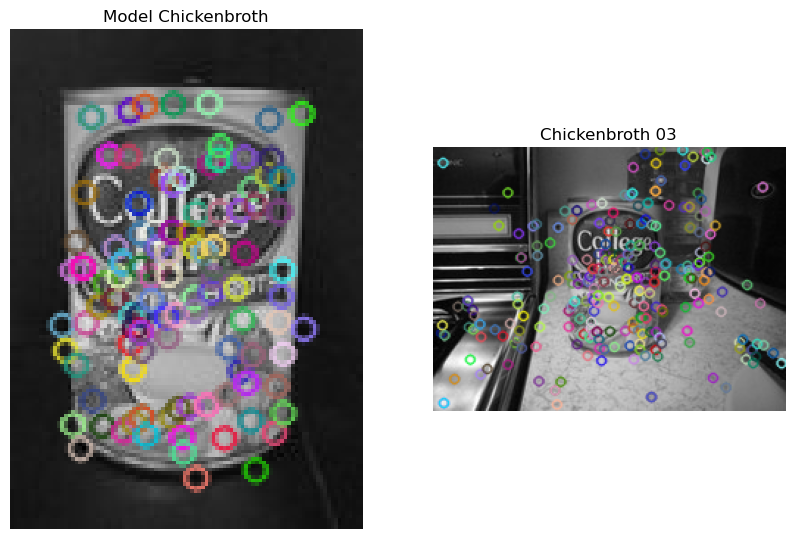
\includegraphics[width=0.5\textwidth]{../output/3.0_sift.png}
    \caption{Descriptor Points on Chickenbroth Model and Counter Images}
    \label{fig:3_1}
\end{figure}

\subsection*{3.1 - Finding Corresponding Points Using SIFT}

\begin{figure}[h!]
    \centering
    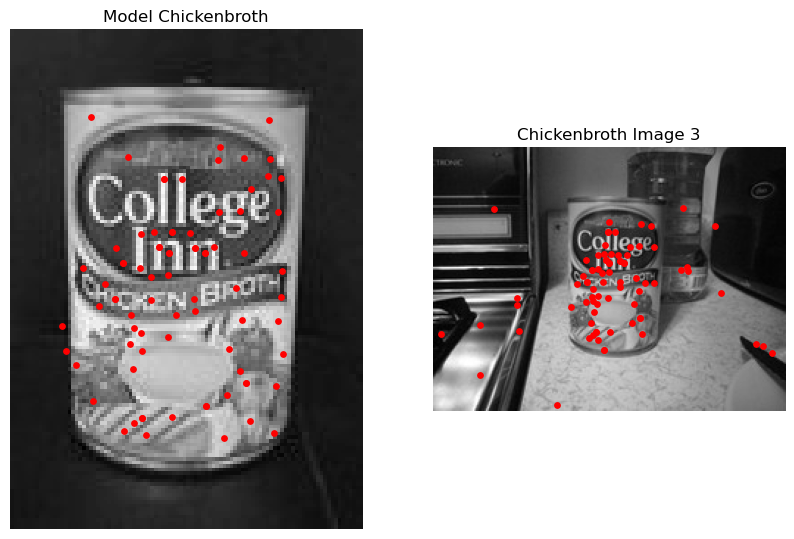
\includegraphics[width=0.5\textwidth]{../output/3.1_cb.png}
    \caption{Corresponding Points on Chickenbroth Model and Counter Images}
    \label{fig:3_1}
\end{figure}

\subsection*{3.2 - Calculating Transformation}

The implemented function to find the homography matrix performs the following steps:
\begin{enumerate}
    \item From given points, constructs the $A$ matrix as seen in lecture. For each point, two rows are defined:
    \[ A = 
    \begin{bmatrix}
        -x & -y & -1 & 0 & 0 & 0 & x'x & x'y & x' \\
        0 & 0 & 0 & -x & -y & -1 & y'x & y'y & y'
    \end{bmatrix}
    \]
    \item Calculate the SVD decomposition of $A$.
    \item Find the minimal singular value and its corresponding column in $V$.
    \item Reshape the column to a $3 \times 3$ matrix $H$ and return it.
\end{enumerate}

The result is projected using the matrix, returned to heterogeneous coordinates and displayed in the image. The result is shown in Figure~\ref{fig:3_2}.

\begin{figure}[h!]
    \centering
    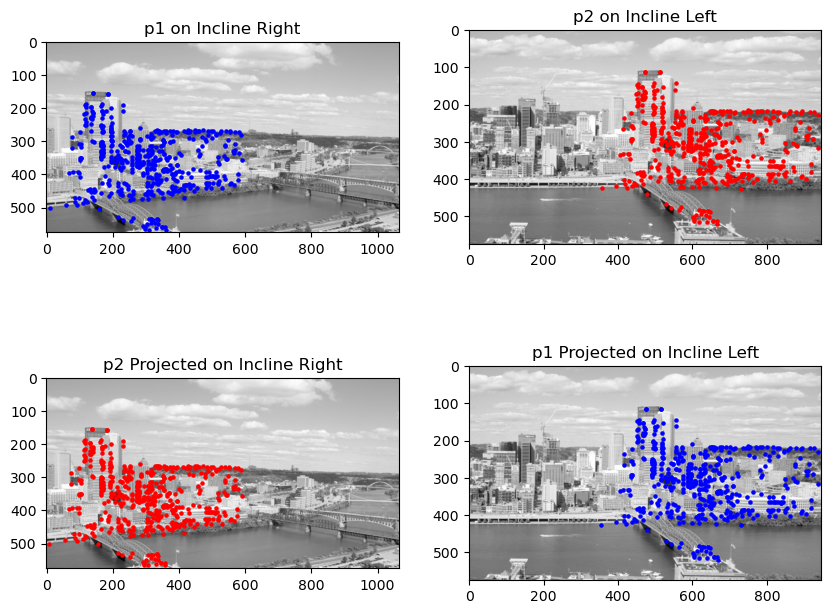
\includegraphics[width=0.8\textwidth]{../output/3.2_incline.png}
    \caption{Homography Transformation of Incline Panorama Images}
    \label{fig:3_2}
\end{figure}

\subsection*{3.3 - Image Warping}

\subsection*{3.4 - Panorama Stitching}

\subsection*{3.5 - Several Image Stitching}

\subsection*{3.6 - RANSAC}

\subsection*{3.7 - Creating Our Own Panorama}

\end{document}